\section{Understanding and Modeling Transient Server Preemptions}

Transient cloud servers, by their very nature have limited availability and are frequently preempted.
These preemptions are akin to fail-stop failures, and are often preceeded by a small advance warning (few seconds) to allow for graceful shutdowns.

Since preemptions can impact the availability, performance, and cost of running applications, in this section, we examine their preemption characteristics.
This modeling is important, because having a model of the availability can be useful in the context of predicting the running times of applications.
Cloud providers offer a large number of servers of different configurations and types.
Since transient server availability is fundamentally tied to supply and demand, the availability of servers of different types can be significantly different. 
Thus, selecting the ``right'' server type is crucial for minimizing the overall costs. 




\subsection{EC2 spot instances}

The earliest form of transient cloud instances.
In addition to having dynamic availability, also have dynamic pricing.
``Classic'' spot instances had price determining the availability, and thus a large amount of work was devoted to bidding and analyzing the prices.

However a recent change to the spot prices no longer allows these assumptions, rendering it impossible to obtain the \emph{exact} availability information from the prices alone.


\subsection{Google Preemptible VMs}

Launched in 2015.
Flat-rate discount of 80\% compared to on-demand servers.
Interesting availability SLA: the maximum lifetime is 24 hours, and can be preempted earlier as well.

In this paper we will look at these preemptible VMs and show how to model their availability.
Given the inability to use EC2 prices, we believe that our approach is more generalizable and robust.

\begin{figure}
  \centering
  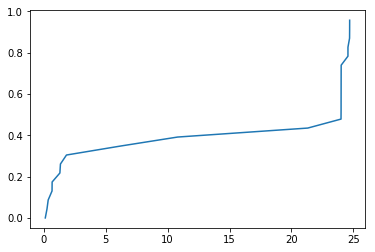
\includegraphics[width=0.4\textwidth]{../data/f20.png}
  \caption{CDF of lifetimes of Google Preemptible Instances }
  \label{fig:gcp1}
\end{figure}

There are some distinguishing characteristics of GCP preemptible VMs that makes their failure modeling challenging.
First is their flat pricing and no other signalling information about their preemption rates (MTBFs) that makes server selection difficult.

\textbf{Modeling Failure Behavior of Preemptible VMs}
CDF is ``sigmoid'' shaped.
$P=R*np.sinh((t-t0)/tau) + C$ with a very low $R=10^{-6}, t_0=12, \tau=0.9, C=0.36$

Basically, this is a mixture of two distributions, the standard exponential distribution, which we call the stabilization rate and an exponentially increasing reclamation rate.

Preemptible VMs have three availability phases.

There are many early deaths, then a period of low failure rates, and then the failure rate is exponential with a positive exponent to enable the cloud provider to reclaim the VMs within the deadline (24 hours in the case of Google's Preemptible VMs).



\subsection{Trade-offs in Server Selection}
% Maybe this can come in the earlier section?

This presents us with many challenges in the cloud-deployment of these jobs.

Cloud providers offer multiple types of instances (VMs), with different hardware configuration (such as number of CPUs and memory size).
The price of cloud servers is related to their hardware configuration, but it may not be strictly proportional to the hardware performance.
For example, a VM with 32 CPUs may not be 32 times the cost of a single CPU VM.


For parallel and distributed applications, the type of servers selected has large implications on their performance.
Consider the case of deploying an application on 8 8-core VMs vs. 16 4-core VMs.
In both cases, the total number of CPU cores is the same.
However, the larger number of VMs requires more communication between the application tasks, and thus may result in performance degradation.
The performance of applications at different cluster configurations depends on their communication patterns and scaling properties. 



Thus, when deploying applications on the cloud, one has to mindful of the cost and performance tradeoff.
However, in the case of transient servers, the story does not stop here. 


In addition to pricing differences, the transient availability of instances \emph{also} differs by type.
Because the availability of a transient VM is broadly determined by the overall supply and demand of the instances of that \emph{particular} type, the ``preemption rate'' of VMs often depends on the type of the instance.



Thus, selecting a transient cloud server involves a complex tradeoff between the cost of servers, their performance, and the preemption-rate.
We develop server selection policies in the next section.





%%% Local Variables:
%%% mode: latex
%%% TeX-master: "paper"
%%% End:
